\documentclass[11pt,a4paper]{article}
\usepackage[utf8]{inputenc}
\usepackage[T1]{fontenc}
\usepackage[english]{babel}
\usepackage{lmodern}
\usepackage{microtype}
\usepackage[a4paper,margin=1.65cm,headheight=20pt]{geometry}
\usepackage{xcolor}
\usepackage{graphicx}
\usepackage{booktabs,tabularx,array,colortbl}
\usepackage{amsmath,amssymb}
\usepackage{multicol}
\usepackage{enumitem}
\usepackage{titlesec}
\usepackage{fancyhdr}
\usepackage{tcolorbox}
\tcbuselibrary{breakable,skins}
\usepackage{tikz}
\usetikzlibrary{arrows.meta,positioning,shapes.geometric,fit,calc,backgrounds}
\usepackage{caption}
\usepackage{hyperref}
\usepackage{parskip}
\usepackage{ragged2e}
\usepackage{setspace}
\usepackage{float}
\usepackage{pdflscape}
\usepackage{eso-pic}

\definecolor{Teal}{HTML}{0E5A5D}
\definecolor{DeepTeal}{HTML}{063D40}
\definecolor{MidTeal}{HTML}{4B898B}
\definecolor{SoftTeal}{HTML}{DCEBEC}
\definecolor{PaleTeal}{HTML}{EEF5F5}
\definecolor{MistTeal}{HTML}{F7FAFA}
\definecolor{Ink}{HTML}{173335}
\definecolor{SoftGray}{HTML}{F4F7F7}
\definecolor{WarmTeal}{HTML}{B8D4D5}
\definecolor{AccentTeal}{HTML}{7BA6A8}

\hypersetup{colorlinks=true,linkcolor=DeepTeal,urlcolor=Teal,citecolor=MidTeal,
  pdftitle={MMALS Science Magazine v5 - English Edition},
  pdfauthor={Guillaume Harbonnier - MMALS Project}}

\pagestyle{fancy}
\fancyhf{}
\fancyhead[L]{\textcolor{Teal}{\small MMALS Science Magazine}}
\fancyhead[R]{\textcolor{Teal}{\small Routes, functions, memory and decision}}
\fancyfoot[C]{\thepage}
\renewcommand{\headrulewidth}{0.4pt}
\renewcommand{\headrule}{\hbox to\headwidth{\color{MidTeal}\leaders\hrule height \headrulewidth\hfill}}

\titleformat{\section}{\color{DeepTeal}\Large\bfseries}{\thesection}{0.6em}{}
\titleformat{\subsection}{\color{Teal}\large\bfseries}{\thesubsection}{0.5em}{}
\titleformat{\subsubsection}{\color{Ink}\normalsize\bfseries}{\thesubsubsection}{0.5em}{}

\newtcolorbox{twelvebox}[1][]{breakable,enhanced,colback=PaleTeal,colframe=Teal,boxrule=0pt,leftrule=2.2pt,arc=0mm,left=4mm,right=4mm,top=3mm,bottom=3mm,title={Age-12 view},fonttitle=\bfseries\sffamily,coltitle=white,colbacktitle=DeepTeal,#1}
\newtcolorbox{engineerbox}[1][]{breakable,enhanced,colback=MistTeal,colframe=MidTeal,boxrule=0pt,leftrule=2.2pt,arc=0mm,left=4mm,right=4mm,top=3mm,bottom=3mm,title={Engineer view},fonttitle=\bfseries\sffamily,coltitle=white,colbacktitle=MidTeal,#1}
\newtcolorbox{researchbox}[1][]{breakable,enhanced,colback=SoftTeal!55,colframe=DeepTeal,boxrule=0pt,leftrule=2.2pt,arc=0mm,left=4mm,right=4mm,top=3mm,bottom=3mm,title={Research view},fonttitle=\bfseries\sffamily,coltitle=white,colbacktitle=DeepTeal,#1}
\newtcolorbox{keybox}[1][]{breakable,enhanced,colback=DeepTeal!5,colframe=Teal,boxrule=0.7pt,arc=0mm,left=4mm,right=4mm,top=3mm,bottom=3mm,title={Key idea},fonttitle=\bfseries\sffamily,coltitle=white,colbacktitle=DeepTeal,#1}
\newtcolorbox{notebox}[1][]{breakable,enhanced,colback=white,colframe=MidTeal,boxrule=0pt,leftrule=1.5pt,arc=0mm,left=3mm,right=3mm,top=2mm,bottom=2mm,#1}
\newtcolorbox{statusbox}[1][]{breakable,enhanced,colback=SoftGray,colframe=DeepTeal,boxrule=0.6pt,arc=0mm,left=4mm,right=4mm,top=3mm,bottom=3mm,title={Scientific status},fonttitle=\bfseries\sffamily,coltitle=white,colbacktitle=DeepTeal,#1}

\newcommand{\mmals}{\textsc{MMALS}}
\newcommand{\codeword}[1]{\texttt{\textcolor{DeepTeal}{#1}}}
\newcommand{\tablehead}[1]{\cellcolor{DeepTeal}\color{white}\bfseries #1}
\newcommand{\smallcaps}[1]{\textsc{#1}}

\begin{document}

% Full-bleed cover, with no blank first page.
\begin{titlepage}
\thispagestyle{empty}
\AddToShipoutPictureBG*{%
  \AtPageLowerLeft{%
    
\includegraphics[width=\paperwidth,height=\paperheight]{assets/MMALS_Science_Magazine_cover.png}%
  }%
}
\begin{tikzpicture}[remember picture,overlay]
  \node[anchor=north west,fill=white,minimum width=8.6cm,minimum height=0.48cm,inner xsep=4pt,inner ysep=2pt,text=DeepTeal,font=\sffamily\bfseries\scriptsize,align=left]
  at ([xshift=1.05cm,yshift=-1.05cm]current page.north west)
  {VOLUME 01 \textbullet\ ISSUE 00 \textbullet\ JUNE 2026};
\end{tikzpicture}
\null
\end{titlepage}
\clearpage

\tableofcontents
\newpage

\section*{Foreword: what this magazine is trying to do}
\addcontentsline{toc}{section}{Foreword: what this magazine is trying to do}

\begin{multicols}{2}
\mmals{} stands for \emph{Mycelium-Inspired Mutualistic Adaptive Learning Systems}. The original intuition is simple to state: instead of asking one shared network to learn everything, can we organise several specialised modules and connect them through a medium that learns which exchanges to select, transform and preserve?

The biological mapping remains strict throughout the magazine. The \textbf{hosts are the trees or other host organisms}. The \textbf{fungal system} is the mycelial medium that connects, transforms and allocates exchanges. The \textbf{mycorrhiza} is the mutualistic interface and relationship between host roots and the fungus. These three objects must not be collapsed into one metaphor.

The analogy is not evidence. It is a machine for generating questions. Why broadcast everywhere if communication has a cost? Why allocate weight to a host that does not contribute? How can a useful exchange remain stable while the system continues learning? Where does memory live: in parameters, routes, functions, distributions, or a combination of them?

The text deliberately uses three reading levels. The age-12 view gives a mental picture. The engineer view shows the objects, equations and code. The research view separates hypotheses, metrics, evidence, limits and the next falsifiable experiment.
\end{multicols}

\begin{keybox}
Read the magazine in the same order as a good engineering investigation: first the story, then the symbols, then the code, then the claim boundary.
\end{keybox}

\newpage
\section{The starting problem: learning without overwriting everything}

\begin{twelvebox}
Imagine a student who first learns cats and dogs, then bicycles and cars, then apples and bananas. After the third lesson, the student recognises bananas perfectly but can no longer recognise cats. The student did not merely add knowledge; part of the earlier knowledge was overwritten.

That is catastrophic forgetting.
\end{twelvebox}

\begin{engineerbox}
In continual learning, a model observes a sequence of tasks or regimes $\mathcal{T}_1,\ldots,\mathcal{T}_K$. Parameters useful for a new task may damage representations required by an older one:
\[
A_{\tau}(\theta_{t+1}) < A_{\tau}(\theta_t), \qquad \tau<t+1.
\]
The key question is not only whether the model learns, but what it destroys while learning.
\end{engineerbox}

\begin{researchbox}
The early MMALS programme reduced the broad ambition to a narrow question: can sparse, persistent, adaptive routing reduce interference relative to a shared model? Later versions separated capacity, freezing, routing, output distillation, latent preservation and functional memory. This versioned progression matters because each mechanism can otherwise be mistaken for the effect of the biological analogy itself.
\end{researchbox}

\section{Tree hosts: several small networks instead of one brain}

\subsection{What is a host?}

\begin{twelvebox}
A host is a small expert. Every host sees the same input, but each can learn a different useful view. One may respond to shape, another to texture, another to orientation, and another to combinations that humans cannot easily name.
\end{twelvebox}

\begin{engineerbox}
Host $i$ is a parametrised function
\[
z_i=g_i(x;\theta_i).
\]
$x$ is the input and $z_i$ is a latent representation. In the simplest notebooks, a host is an MLP:
\[
\texttt{Linear}\rightarrow\texttt{ReLU}\rightarrow\texttt{Linear}\rightarrow\texttt{ReLU}.
\]
\end{engineerbox}

\subsection{Linear, ReLU and the MLP}

\begin{twelvebox}
A \texttt{Linear} layer mixes numbers. ReLU is an on-off gate: negative values become zero, positive values continue. Putting ReLU between two linear layers lets the mini-network learn much richer rules than one linear map alone.
\end{twelvebox}

\begin{engineerbox}
A linear layer computes $y=Wx+b$. A small MLP can be written
\[
g_i(x)=W_{i,2}\,\sigma(W_{i,1}x+b_{i,1})+b_{i,2},
\]
where $\sigma(u)=\max(0,u)$ for ReLU. Training adjusts $W$ and $b$ by gradient descent.
\end{engineerbox}

\begin{researchbox}
Multiple hosts do not automatically imply genuine specialisation. Evidence requires host ablations, route swaps, equal-capacity controls, contribution estimates, representation separation and cross-seed stability. A larger host bank may win only because it contains more parameters.
\end{researchbox}

\newpage
\section{The fungal medium: route, transform and combine}

% Native redraw replacing the previously cropped figure.
\begin{figure}[H]
\centering
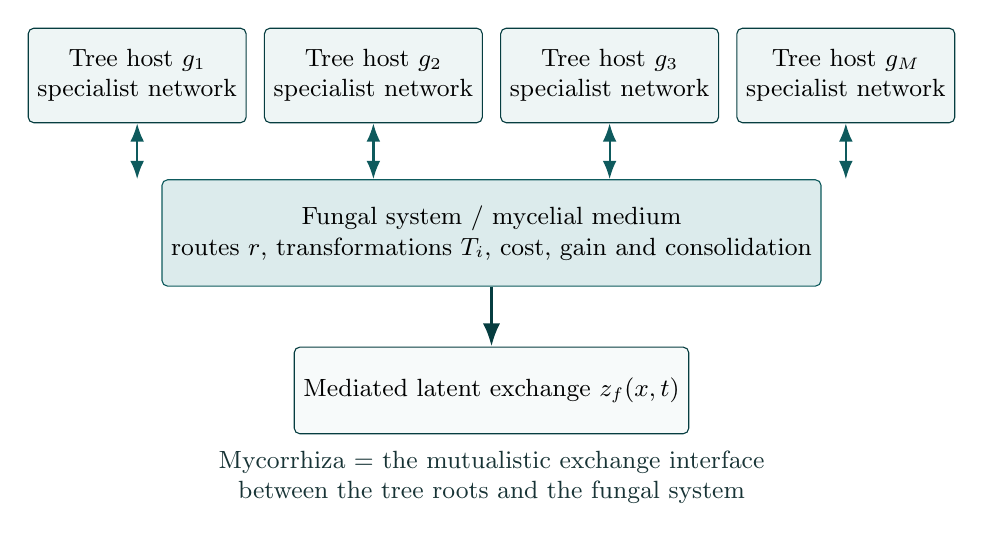
\begin{tikzpicture}[x=1cm,y=1cm,>=Latex, font=\small]
  \tikzset{tree/.style={draw=DeepTeal,rounded corners=2pt,fill=PaleTeal,minimum width=2.6cm,minimum height=1.2cm,align=center},
           fungal/.style={draw=Teal,rounded corners=2pt,fill=SoftTeal,minimum width=7.6cm,minimum height=1.35cm,align=center},
           latent/.style={draw=DeepTeal,rounded corners=2pt,fill=MistTeal,minimum width=4.2cm,minimum height=1.1cm,align=center}}
  \node[tree] (h1) at (-4.5,2.4) {Tree host $g_1$\\specialist network};
  \node[tree] (h2) at (-1.5,2.4) {Tree host $g_2$\\specialist network};
  \node[tree] (h3) at (1.5,2.4) {Tree host $g_3$\\specialist network};
  \node[tree] (hm) at (4.5,2.4) {Tree host $g_M$\\specialist network};
  \node[fungal] (f) at (0,0.4) {Fungal system / mycelial medium\\routes $r$, transformations $T_i$, cost, gain and consolidation};
  \node[latent] (z) at (0,-1.6) {Mediated latent exchange $z_f(x,t)$};
  \foreach \h in {h1,h2,h3,hm}{\draw[<->,thick,Teal] (\h.south) -- (\h.south |- f.north);}
  \draw[->,very thick,DeepTeal] (f) -- (z);
  \node[align=center,text=Ink] at (0,-2.7) {Mycorrhiza = the mutualistic exchange interface\\between the tree roots and the fungal system};
\end{tikzpicture}
\caption{The disciplined biological mapping. Tree hosts emit representations; the fungal system transforms and allocates exchanges; mycorrhiza names the host--fungus interface. This native redraw replaces the cropped image reused from the mathematical note.}
\label{fig:forest-redraw}
\end{figure}

\begin{landscape}
\thispagestyle{empty}
\begin{figure}[p]
\centering
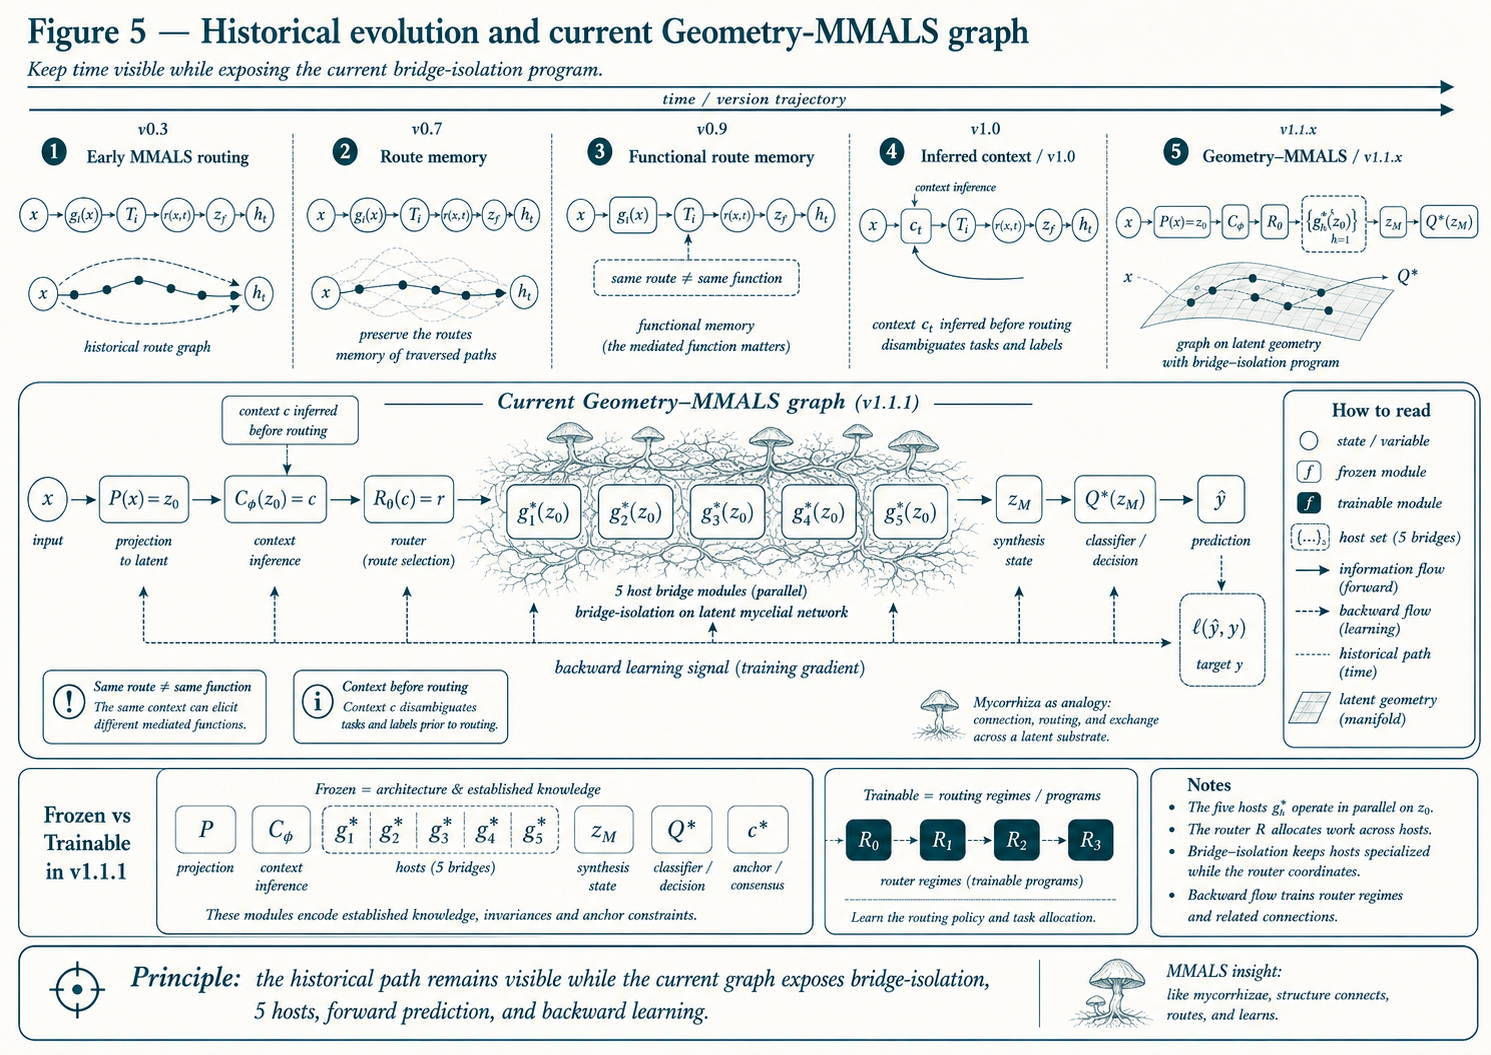
\includegraphics[width=0.985\linewidth,height=0.92\textheight,keepaspectratio]{assets/figure_05_historical_current_graph.png}
\caption{Historical evolution and the current Geometry-MMALS graph. The diagram keeps time visible while exposing five hosts, forward prediction, backward learning, frozen modules and trainable routing treatments.}
\label{fig:historical-current-graph}
\end{figure}
\end{landscape}
\clearpage

\subsection{The transformation $T_i$}

\begin{twelvebox}
Tree hosts do not necessarily speak the same internal language. $T_i$ acts as a translator: it converts the signal from host $i$ into a common space where signals can be combined.
\end{twelvebox}

\begin{engineerbox}
The fungal transformation is
\[
T_i:\mathbb{R}^{d_i}\rightarrow\mathbb{R}^{d}.
\]
It may be an identity map, a linear projection $T_i(z)=W_i z+b_i$, or a small MLP. It can align dimensions, filter, amplify or reshape a host representation. It may include normalisation, but it is not merely normalisation.
\end{engineerbox}

\begin{researchbox}
$T_i$ gives functional meaning to the route. A route can remain numerically unchanged while $T_i$ or $g_i$ drifts. Identical routing coefficients therefore do not certify identical computation.
\end{researchbox}

\newpage
\section{The probability simplex: the space of all routing recipes}

\subsection{Why is a route a distribution?}

A route over $M$ hosts is a vector
\[
r=(r_1,\ldots,r_M), \qquad r_i\geq0, \qquad \sum_i r_i=1.
\]
The coefficients form a finite resource budget. The fungal system cannot allocate more than 100\% in total.

% Native simplex redraw replacing the cropped source image.
\begin{figure}[H]
\centering
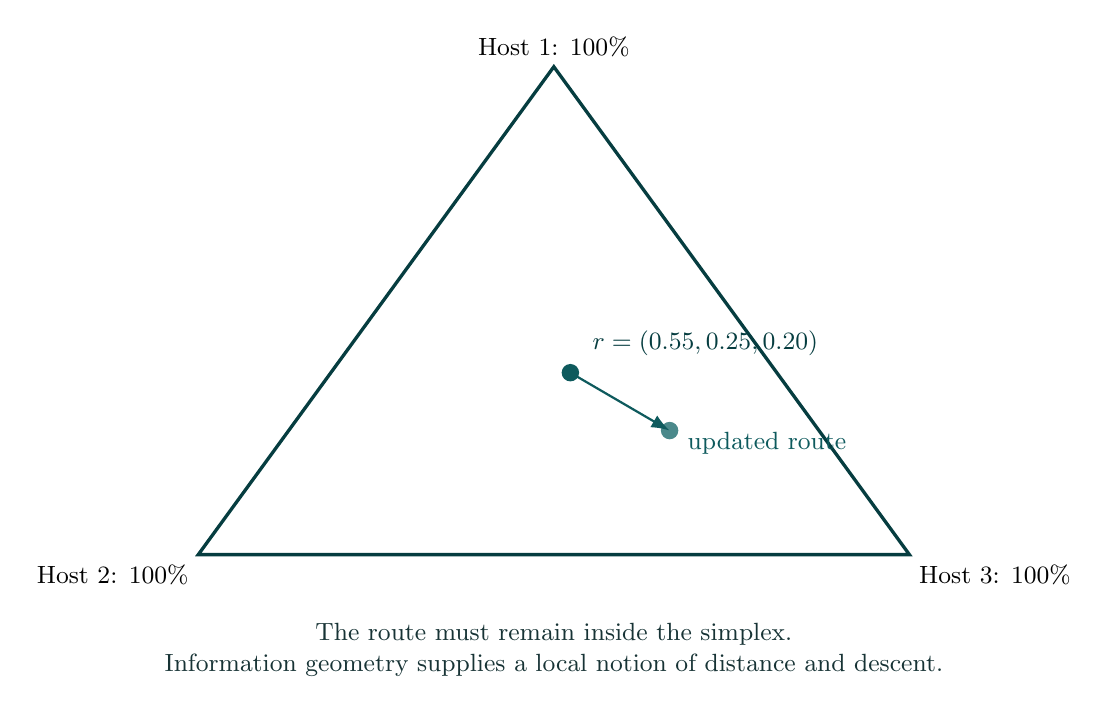
\begin{tikzpicture}[scale=1.05,>=Latex,font=\small]
  \coordinate (A) at (0,4.8);
  \coordinate (B) at (-4.3,-1.1);
  \coordinate (C) at (4.3,-1.1);
  \draw[very thick,DeepTeal] (A)--(B)--(C)--cycle;
  \node[above] at (A) {Host 1: 100\%};
  \node[below left] at (B) {Host 2: 100\%};
  \node[below right] at (C) {Host 3: 100\%};
  \coordinate (p) at (0.2,1.1);
  \coordinate (q) at (1.4,0.4);
  \fill[Teal] (p) circle (3pt);
  \fill[MidTeal] (q) circle (3pt);
  \draw[->,thick,Teal] (p) -- (q);
  \node[right,text=DeepTeal] at ($(p)+(0.15,0.35)$) {$r=(0.55,0.25,0.20)$};
  \node[right,text=Teal] at ($(q)+(0.1,-0.15)$) {updated route};
  \node[align=center,text=Ink] at (0,-2.25) {The route must remain inside the simplex.\\Information geometry supplies a local notion of distance and descent.};
\end{tikzpicture}
\caption{The routing simplex. Vertices correspond to one-host routing; interior points are mixtures. This vector redraw fixes the clipping of the figure extracted from the earlier PDF.}
\label{fig:simplex-redraw}
\end{figure}

\begin{twelvebox}
Think of a recipe that must always total 100\%. A point near one corner uses mostly one host. A point near the centre spreads attention across several hosts.
\end{twelvebox}

\begin{engineerbox}
The router often produces logits $a_i$ and applies softmax:
\[
r_i=\frac{\exp(a_i/\tau)}{\sum_j\exp(a_j/\tau)}.
\]
A low temperature $\tau$ makes routing sharper; a high temperature makes it more diffuse.
\end{engineerbox}

\subsection{Entropy and the carbon-cost metaphor}

\[
H(r)=-\sum_i r_i\log(r_i+\varepsilon).
\]
High entropy means broad allocation. Low entropy means selective routing. In the early MMALS notebooks, entropy is used as a proxy for communication or carbon cost. This is a modelling metaphor, not a literal biological measurement.

\begin{keybox}
The simplex gives the geometry of valid recipes. The mycelium analogy gives an economy of recipes: allocation, cost, exchange and reinforcement.
\end{keybox}

\newpage
\section{The mediated latent representation}

Each host produces $g_i(x)$, the fungal system transforms it with $T_i$, and the route combines the transformed signals:
\[
z_f(x,t)=\sum_{i=1}^{M}r_i(x,t)\,T_i(g_i(x)).
\]
A readout or head then predicts
\[
\hat y=h_t(z_f) \quad\text{or}\quad \hat y=Q(z_M).
\]

\begin{twelvebox}
The latent representation is the internal idea formed before the final answer. It is neither the raw image nor the class label. It is the compact internal description used to decide.
\end{twelvebox}

\begin{engineerbox}
The mediated latent is the first place where host computation, fungal transformation and routing all meet. That is why preserving it can carry more functional information than preserving route coefficients alone.
\end{engineerbox}

\section{How MMALS learns: forward flow and backward credit}

The forward flow is
\[
x\rightarrow g_i(x)\rightarrow T_i(g_i(x))\rightarrow r(x,t)\rightarrow z_f\rightarrow h_t(z_f)\rightarrow\hat y.
\]
After comparing $\hat y$ with the target $y$, the loss is differentiated backward through the head, mixture, route, transformations and hosts.

\begin{engineerbox}
A generic training step is:
\begin{verbatim}
optimizer.zero_grad()
logits, cache = model(x, context)
loss = task_loss(logits, y) + fungal_terms(cache)
loss.backward()
optimizer.step()
\end{verbatim}
The call \codeword{loss.backward()} computes gradients. \codeword{optimizer.step()} applies the parameter update.
\end{engineerbox}

\subsection{The fungal objective}

A representative v0.3-style loss is
\[
\mathcal{L}=\mathcal{L}_{\text{task}}
+\lambda_H H(r)
+\lambda_M\|z_f\|_2^2
+\lambda_G\sum_i r_i\max(0,\epsilon_G-G_i).
\]
The leave-one-host-out contribution is
\[
G_i=\mathcal{L}_{\text{without }i}-\mathcal{L}_{\text{full}}.
\]
If $G_i>0$, removing host $i$ makes performance worse, so the host contributed. If $G_i<0$, that host was unnecessary or harmful for the current batch.

\begin{researchbox}
Early mutualistic credit was noisy because hosts were immature. v0.4 therefore introduced warm-up, delayed mutualism and soft consolidation. The lesson is general: a biologically inspired objective can still fail because of training dynamics.
\end{researchbox}

\newpage
\section{Supervised learning, inferred context and unsupervised learning}

\subsection{Does learning always require labels?}

No. It requires a corrective signal, but not always a human class label.

\begin{tabularx}{\textwidth}{>{\raggedright\arraybackslash}p{3cm}X}
\toprule
\tablehead{Learning mode} & \tablehead{What provides the corrective signal?}\\
\midrule
Supervised & A label $y$, such as ``shoe'' or ``class 4''.\\
Self-supervised & A task constructed from the data, such as predicting a masked part or matching two views.\\
Unsupervised & Structure such as clusters, density, reconstruction or contrast.\\
Reinforcement learning & Reward, cost, delayed outcome or constraint violation.\\
\bottomrule
\end{tabularx}

The immediate MMALS transition is not fully unsupervised learning. It is the removal of the explicit task identifier while keeping labels for the downstream task.

\subsection{Inferred context}

Instead of being told ``this is task 3'', the system estimates
\[
q(c\mid x).
\]
For example,
\[
q(c\mid x)=(0.80,0.15,0.05).
\]
The model is 80\% confident in context 1, but it keeps alternatives rather than pretending certainty.

\begin{twelvebox}
You enter a classroom and see rulers, triangles and equations. Nobody tells you the subject, but you infer that it is probably mathematics. That is inferred context.
\end{twelvebox}

\begin{researchbox}
Removing task identity changes the scientific problem. The model must infer the situation, quantify ambiguity and avoid task leakage through a task-specific head. This is one reason the later Geometry-MMALS line moves toward a shared readout.
\end{researchbox}

\newpage
\section{Distillation: learning the new without betraying the old}

Distillation keeps a frozen teacher snapshot and asks the current student to remain close to the teacher on old behaviour.
\[
\mathcal{L}_{\text{distill}}=T^2D_{\mathrm{KL}}\!\left(p_{\text{teacher}}\parallel p_{\text{current}}\right).
\]

\begin{twelvebox}
The new student is allowed to learn a new lesson, but an old teacher checks that the student has not changed the meaning of earlier answers too much.
\end{twelvebox}

Distillation can preserve several layers:
\begin{itemize}[leftmargin=1.4em]
\item \textbf{output distillation}: preserve final predictive distributions;
\item \textbf{route distillation}: preserve routing patterns;
\item \textbf{latent distillation}: preserve mediated internal computations;
\item \textbf{transformation regularisation}: preserve aspects of $T_i$ or its local sensitivity.
\end{itemize}

\begin{keybox}
Replay stores old examples or regenerates them. Distillation stores a behaviour. They are related, but they are not the same mechanism.
\end{keybox}

\section{From one memory point to a memory law}

% Native memory-law redraw replacing the truncated source image.
\begin{figure}[H]
\centering
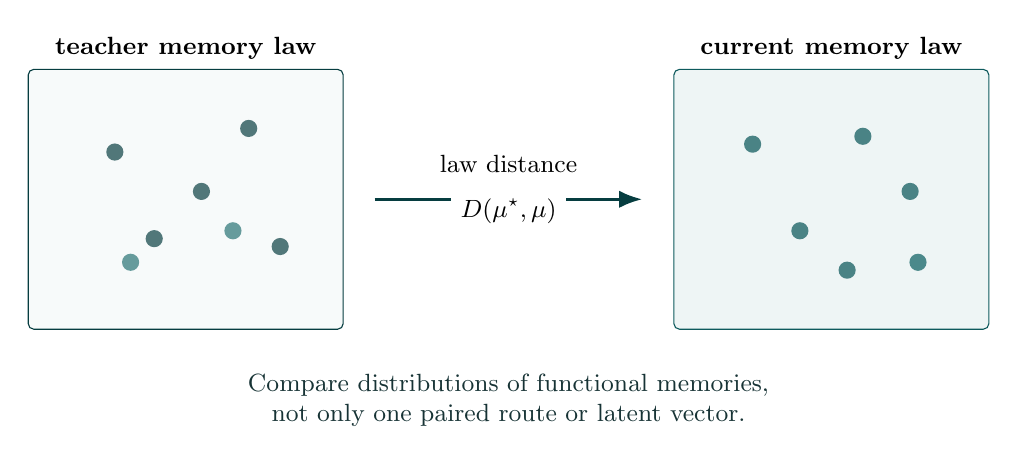
\begin{tikzpicture}[>=Latex,font=\small]
  \node[draw=DeepTeal,rounded corners=2pt,minimum width=4cm,minimum height=3.3cm,fill=MistTeal,label=above:{\bfseries teacher memory law}] (a) at (-4.1,0) {};
  \node[draw=Teal,rounded corners=2pt,minimum width=4cm,minimum height=3.3cm,fill=PaleTeal,label=above:{\bfseries current memory law}] (b) at (4.1,0) {};
  \foreach \x/\y in {-5.0/0.6,-4.5/-0.5,-3.9/0.1,-3.3/0.9,-2.9/-0.6}{\fill[DeepTeal!70] (\x,\y) circle (3.1pt);}
  \foreach \x/\y in {-4.8/-0.8,-3.5/-0.4}{\fill[MidTeal!85] (\x,\y) circle (3.1pt);}
  \foreach \x/\y in {3.1/0.7,3.7/-0.4,4.5/0.8,5.1/0.1,4.3/-0.9}{\fill[Teal!75] (\x,\y) circle (3.1pt);}
  \fill[MidTeal] (5.2,-0.8) circle (3.1pt);
  \draw[->,very thick,DeepTeal] (-1.7,0) -- (1.7,0);
  \node[align=center,fill=white] at (0,0.45) {law distance};
  \node[align=center,fill=white] at (0,-0.15) {$D(\mu^{\star},\mu)$};
  \node[align=center,text=Ink] at (0,-2.55) {Compare distributions of functional memories,\\not only one paired route or latent vector.};
\end{tikzpicture}
\caption{Teacher and current functional-memory laws. This native redraw fixes the cropping of the earlier extracted figure.}
\label{fig:law-redraw}
\end{figure}

A context induces a distribution of route states, latent states and output distributions over many samples. We can define
\[
\mu^{z,\Theta}_{\tau}=\mathcal{L}_{X\sim P_\tau}\bigl(z_f^{\Theta}(X,\tau)\bigr).
\]
Pointwise drift asks whether paired samples changed. Law-level drift asks whether the whole distribution changed.

\begin{twelvebox}
A single marble can look unchanged while the composition of the jar changes. One route is a marble; the route law is the jar.
\end{twelvebox}

\newpage
\section{The central internal discovery: same route, different function}

The v0.9 diagnostic non-implication is
\[
r_{\text{current}}(x,t)\approx r_{\text{teacher}}(x,t)
\not\Rightarrow
z_{f,\text{current}}(x,t)\approx z_{f,\text{teacher}}(x,t).
\]
If the route is $[1,0,0]$ in both models but the first host or transformation has changed, then route drift can be zero while functional latent drift is positive.

\begin{tabularx}{\textwidth}{p{2.2cm}X}
\toprule
\tablehead{Metric} & \tablehead{Question answered}\\
\midrule
$D_r$ & Did the selected route change?\\
$D_z$ & Did the mediated latent computation change?\\
$D_y$ & Did final predictive behaviour change?\\
$D_T$ & Did transformed host outputs change in isolation?\\
$D_J$ & Did local sensitivity or Jacobian structure change?\\
\bottomrule
\end{tabularx}

\begin{keybox}
Memory is not merely the route identity. It is the function computed through the route, under the data distribution and context.
\end{keybox}

\section{The experimental story: v0.1 to v0.14.x}

\begin{tabularx}{\textwidth}{p{1.45cm}X X}
\toprule
\tablehead{Version} & \tablehead{Question} & \tablehead{Lesson carried forward}\\
\midrule
v0.1 & Can persistent structural paths reduce forgetting? & Promising toy signal; not evidence for a fungal mechanism.\\
v0.2 & Does the result survive fairer baselines and capacity checks? & Capacity and freezing must be separated from routing.\\
v0.3 & Can the medium have its own cost and mutualistic objective? & The fungal medium became explicit, but training was unstable.\\
v0.4 & Does warm-up and delayed mutualism help? & Specialisation alone is not memory.\\
v0.5--0.6 & Do route memory and output distillation stabilise learning? & Functional behaviour matters more than route identity alone.\\
v0.7--0.9 & Does preserving mediated latent function matter? & Route topology is not the memory object.\\
v0.11 & Is there a real advantage against known CL baselines? & Comparative evidence must be hardened and cost-aware.\\
v0.12--0.13.1 & Does transformation geometry co-drift? & Strong geometry regularisation may over-constrain plasticity.\\
v0.14.x & Can context and head selection move beyond explicit task IDs? & Context inference and shared readout become central.\\
\bottomrule
\end{tabularx}

\newpage
\section{How to read the code in the notebooks}

A useful reading order is:
\begin{enumerate}[leftmargin=1.6em]
\item \textbf{Libraries}: PyTorch, torchvision, NumPy, pandas and matplotlib.
\item \textbf{Dataset builder}: how sequential tasks and replay batches are constructed.
\item \textbf{Model classes}: hosts, transformations, router, context model and readout.
\item \textbf{Forward method}: the exact computation path.
\item \textbf{Loss terms}: the scientific hypotheses made executable.
\item \textbf{Training loop}: what is frozen, what is updated and when.
\item \textbf{Evaluation}: accuracy, forgetting, drift, route entropy and audit gates.
\end{enumerate}

\begin{engineerbox}
The most informative lines are rarely the imports. They are the forward pass, the loss construction, the parameter masks, the evaluation timing and the automatic claim gates.
\end{engineerbox}

\section{Continual Learning: stability versus plasticity}

A continual learner must be stable enough to preserve useful old functions and plastic enough to learn new ones.

\begin{tabularx}{\textwidth}{p{3.2cm}X}
\toprule
\tablehead{Method family} & \tablehead{Core strategy}\\
\midrule
Regularisation & Penalise changes judged important for old tasks, as in EWC or SI.\\
Distillation & Preserve teacher behaviour on old contexts.\\
Replay & Rehearse stored or generated past samples.\\
Expansion & Add modules or freeze old columns, as in PNN-style methods.\\
Sparse MoE & Route inputs to a subset of experts.\\
MMALS & Combine modular hosts, fungal transformation, functional memory and context-aware routing.\\
\bottomrule
\end{tabularx}

The comparative harness must include tuned baselines, joint-training upper bounds, replay-memory accounting and parameter matching. Otherwise a positive result may be reputationally fragile.

\newpage
\section{From Continual Learning to Reinforcement Learning}

Continual Learning asks: how can a model learn a sequence without forgetting? Reinforcement Learning asks: what should the system do now to improve future outcomes?

A sequential decision is represented by
\[
(s_t,a_t,r_t,s_{t+1}).
\]
In MMALS, an action may be a route, host coalition, memory retrieval, computation budget, abstention or request for more evidence.

\begin{twelvebox}
CL is learning several school subjects without forgetting the first ones. RL is deciding which move to make in a game so that the final outcome is good.
\end{twelvebox}

\begin{researchbox}
RL is justified only when a current routing decision changes future host competence, memory, cost or candidate availability. If consequences are effectively one-step, a transparent energy selector or contextual bandit may be sufficient.
\end{researchbox}

\section{Multiple goals and goal-conditioned policies}

A route that maximises accuracy may be poor for retention, cost, stability or ecosystem specialisation. The goal vector can be written
\[
g=(w_A,w_R,w_C,w_D,w_S).
\]

\begin{tabularx}{\textwidth}{p{2.2cm}X}
\toprule
\tablehead{Goal} & \tablehead{Primary preference}\\
\midrule
A & Maximise accuracy.\\
B & Maximise retention and weakest-task performance.\\
C & Minimise compute, memory and latency cost.\\
D & Maximise stability under drift.\\
E & Promote useful ecosystem specialisation.\\
\bottomrule
\end{tabularx}

A goal-conditioned energy can compare admissible routes:
\[
E_\theta(\varrho\mid s,g)=
 w_A\widehat L_{\mathrm{task}}+w_R\widehat L_{\mathrm{ret}}+w_C\widehat C
 +w_D\widehat D-w_S\widehat U_{\mathrm{spec}}+\cdots
\]

\newpage
\section{Forward--backward control and the TPUT loop}

Forward reasoning asks which futures are reachable from the current state. Backward reasoning asks which states are compatible with the desired future. Their intersection guides action selection.

\begin{twelvebox}
In a maze, forward reasoning imagines where each path leads. Backward reasoning starts at the exit and asks which corridors can reach it.
\end{twelvebox}

The minimal TPUT-style loop is:
\begin{enumerate}[leftmargin=1.6em]
\item observe;
\item represent;
\item infer context belief;
\item propose routes;
\item evaluate cost, risk and future effects;
\item commit or abstain;
\item execute;
\item observe outcome;
\item update permitted components;
\item store, compile and audit.
\end{enumerate}

\section{The five memory levels in MMALS}

\begin{tabularx}{\textwidth}{p{3.2cm}X}
\toprule
\tablehead{Memory level} & \tablehead{What is preserved?}\\
\midrule
Route memory & Which hosts and paths were allocated.\\
Latent memory & Which mediated internal representation was produced.\\
Output memory & How the system behaved at the final readout.\\
Transformation memory & How each host signal was translated.\\
Policy memory & How the system selected actions under a goal.\\
\bottomrule
\end{tabularx}

A second distinction separates \textbf{reconstructive memory}, which supports replay and audit, from \textbf{synthetic memory}, which stores cheaper prototypes, macro-routes or compiled summaries.

\newpage
\section{Uncertainty, calibration and the right not to know}

Accuracy does not tell us whether probabilities are trustworthy. A system can be correct on average and dangerously overconfident on difficult cases.

Relevant notions include calibration error, entropy, out-of-distribution detection, selective prediction, abstention and conformal coverage.

\begin{keybox}
A safe system must be allowed to say: ``I do not know enough to commit.''
\end{keybox}

\section{Metric, protocol and claim verification}

A result can be misleading even when the code runs. Three verification layers are therefore useful:

\begin{tabularx}{\textwidth}{p{3.1cm}X}
\toprule
\tablehead{Verifier} & \tablehead{Question}\\
\midrule
Metric evaluator & Is the quantity computed correctly and at the correct evaluation time?\\
Protocol verifier & Is the comparison fair, leak-free, seed-controlled and resource-matched?\\
Claim verifier & Does the written statement stay inside what the evidence supports?\\
\bottomrule
\end{tabularx}

A smoke run validates execution. It does not qualify a scientific claim. A diagnostic result may reveal mechanism without establishing operational superiority.

\section{Causality, ablations and real specialisation}

Frequent host use is not proof of causal value. Relevant interventions include host removal, route swaps, candidate permutation, representation collapse, frozen-host controls and equal-parameter baselines.

\[
G_i=\mathcal L_{\text{without }i}-\mathcal L_{\text{full}}
\]
is a local contribution proxy. Stronger ecosystem-level contribution also accounts for future retention, cost, drift, calibration and audit value.

\newpage
\section{Geometry of routes and functions}

The simplex is more than a convenient constraint. It is a space in which routes move. Geometry asks:
\begin{itemize}[leftmargin=1.4em]
\item what distance separates two routes or two memory laws?
\item are updates locally continuous?
\item do nearby contexts induce nearby functional routes?
\item where do abrupt regime changes occur?
\item does a geometric regulariser improve control or only decorate the analysis?
\end{itemize}

Candidate tools include Jensen--Shannon divergence, Fisher information, natural gradient, mirror descent, optimal transport, covariance geometry and local perturbation maps.

\begin{researchbox}
Geometry earns its place only if it improves prediction, control, diagnosis or claim precision relative to simpler baselines.
\end{researchbox}

\section{Unsupervised and self-supervised context discovery}

A future branch may learn perceptual representations or pseudo-contexts without human task IDs. Possible tools include contrastive learning, clustering, predictive coding and change-point detection.

The immediate role is not to remove all supervision. It is to improve the representation and inference of context:
\[
x\rightarrow e(x)\rightarrow q(c\mid x).
\]

\section{Quantum-inspired memory: a hypothesis, not a promise}

A later MMALS-QI branch represents route-function uncertainty with positive semidefinite trace-one matrices:
\[
\rho\succeq0,\qquad \mathrm{Tr}(\rho)=1.
\]
Classical routing is the diagonal case $\rho_R=\mathrm{diag}(r_1,\ldots,r_H)$. Off-diagonal structure is a classical modelling hypothesis about interactions, not physical quantum entanglement.

\begin{statusbox}
No quantum advantage is claimed. The branch is admissible only if it beats diagonal routing, covariance or Gram alternatives under matched cost and parameter budgets.
\end{statusbox}

\newpage
\section{RC2O: recognising context before routing}

RC2O addresses the question that becomes unavoidable once the task ID is removed:
\[
x\rightarrow q(c\mid x)\rightarrow r(x,c).
\]
A useful memory is operationally useless if the wrong context activates it.

\subsection{A history of successive repairs}

\begin{tabularx}{\textwidth}{p{2.2cm}X X}
\toprule
\tablehead{Stage} & \tablehead{Problem exposed} & \tablehead{Repair direction}\\
\midrule
Early context selection & Task identity was explicit or too clean. & Infer context and measure uncertainty.\\
Dual-anchor selectors & One score was brittle near weak boundaries. & Combine complementary evidence.\\
Veto and ambiguity guards & Average accuracy hid unsafe local decisions. & Add clean-context vetoes and ambiguity locks.\\
Multi-dataset qualification & MNIST-family success did not imply portability. & Test external and harder regimes.\\
Stable--plastic memory & Old context retention remained weak on CORe50. & Preserve both adaptable and stationary evidence.\\
Per-sample fusion repair & A batch-level prototype posterior was copied across mixed replay samples. & Produce context evidence per sample and repair the training path.\\
\bottomrule
\end{tabularx}

\section{The RC2O-8D benchmark: eight regimes, not eight decorative scores}

The 8D scaffold is intended to expose different failure modes rather than produce one leaderboard number.

\begin{tabularx}{\textwidth}{p{3.1cm}X}
\toprule
\tablehead{Dataset or regime} & \tablehead{Main stressor}\\
\midrule
MNIST & Basic retention and mechanism debugging.\\
FashionMNIST & Weaker visual boundaries.\\
RotatedMNIST & Continuous geometric context.\\
PermutedMNIST & Severe representational change.\\
SplitCIFAR10 & External image bridge and stronger feature complexity.\\
SplitCIFAR100 & Fine-grained classes and readout pressure.\\
CORe50 & Sessions, objects, recency and realistic context drift.\\
Eighth protocol regime & Cross-regime candidate selection and goal-conditioned audit, depending on the executed scaffold version.\\
\bottomrule
\end{tabularx}

The magazine must distinguish \emph{qualified}, \emph{diagnostic}, \emph{smoke}, \emph{paused} and \emph{unexecuted} status. Those words are part of the evidence, not editorial decoration.

\newpage
\section{CORe50: old memory improves, but fusion still fails}

RC2O-v2.3.1 produced a meaningful but non-promotable result. Stable--plastic training improved old-context recognition, weakest-task retention, class coverage and forgetting. However, recent-task accuracy regressed beyond tolerance.

The strongest internal component achieved context top-1 accuracy of approximately $0.7692$, while the deployed fused posterior reached only $0.4788$. Average fusion weights were about 98.4\% single-input, 1.1\% plastic and 0.5\% stable.

\begin{twelvebox}
Several advisers had useful evidence, but the decision gate listened almost entirely to one adviser. The problem was not lack of knowledge. It was the fusion of knowledge.
\end{twelvebox}

\begin{researchbox}
The failure was interpreted as a training-interface problem, not proof that prototype evidence was useless. The component results showed the opposite.
\end{researchbox}

\section{RC2O-v2.3.2: repair fusion without rewriting MMALS}

The repair is local. It preserves the host networks, fungal transformations, router, global readout, replay budget and frozen external visual representation.

\subsection{Three evidence families per sample}

\begin{enumerate}[leftmargin=1.6em]
\item \textbf{Single-input branch}: the learned context encoder, already per sample.
\item \textbf{Plastic branch}: prototypes in current learned feature and mediated-latent coordinates.
\item \textbf{Stable branch}: prototypes in a stationary input representation.
\end{enumerate}

Per-sample diagonal-Gaussian energy is
\[
E_c(x)=\frac1d\sum_{j=1}^{d}
\left[
\frac{(x_j-\mu_{c,j})^2}{\max(\sigma_{c,j}^2,\epsilon)}
+\log\max(\sigma_{c,j}^2,\epsilon)
\right],
\]
and
\[
q_{\mathrm{proto}}(c\mid x)=
\frac{\exp(-E_c(x)/\tau)}{\sum_k\exp(-E_k(x)/\tau)}.
\]
Each sample in a mixed replay batch can now receive a different posterior.

\subsection{Stable and plastic are not synonyms for old and new}

The plastic bank follows the current learned geometry and can adapt quickly, but it may drift. The stationary stable bank stores statistics in the representation entering MMALS, outside the continually updated context encoder and mediated latent space.

A fixed control uses
\[
q_{\mathrm{deploy}}=0.10q_{\mathrm{single}}+0.35q_{\mathrm{plastic}}+0.55q_{\mathrm{stable}}.
\]
Adaptive fusion adds a residual prior floor so that no branch can suppress the others completely.

\subsection{Repair the learning path too}

In v2.3.1, non-legacy candidates did not always receive the main current-task gradient through the same deployed posterior used at inference. v2.3.2 aligns training and evaluation paths.

\begin{statusbox}
RC2O-v2.3.2 is an unexecuted diagnostic ablation design. It reports no v2.3.2 experimental success. Promotion depends on predefined old-context, recent-task, branch-gap, fusion-collapse and stationary-bank gates.
\end{statusbox}

\newpage
\section{RC2O, Geometry-MMALS and TPUT: three complementary questions}

\begin{tabularx}{\textwidth}{p{3.4cm}X}
\toprule
\tablehead{Branch} & \tablehead{Primary question}\\
\midrule
RC2O & Which context or regime am I in?\\
Geometry-MMALS & Does context structure meaningfully organise routes and functions?\\
TPUT / RL & Which route or action should be selected under the current goal and future consequences?\\
\bottomrule
\end{tabularx}

Together they form
\[
\text{perceive}\rightarrow\text{infer context}\rightarrow\text{route}\rightarrow\text{compute}\rightarrow\text{remember}\rightarrow\text{act}\rightarrow\text{verify}.
\]

\section{Geometry-MMALS G1: v1.1.0 results and the next decisive test}

\begin{figure}[H]
\centering
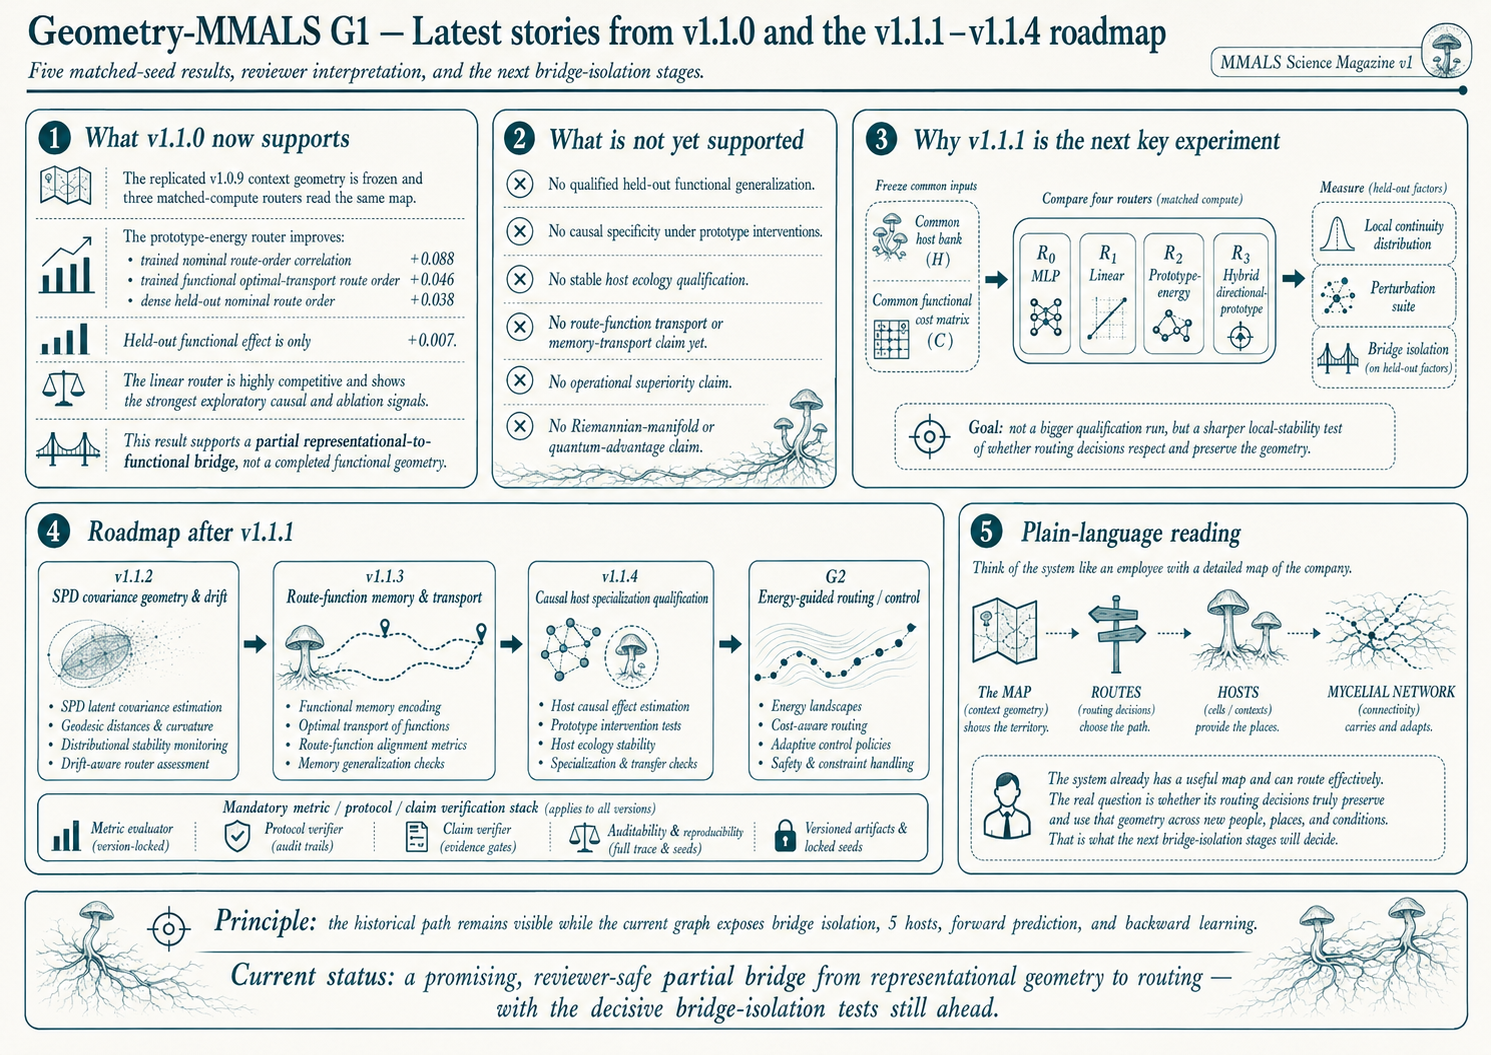
\includegraphics[width=0.98\linewidth]{assets/figure_geometry_g1_latest_stories.png}
\caption{Geometry-MMALS G1 summary: matched routers, supported results, blocked claims and the v1.1.1--v1.1.4 roadmap.}
\end{figure}

v1.1.0 froze the replicated context geometry and compared three matched-compute routers: MLP, linear and prototype-energy. The prototype improved trained nominal route-order correlation and trained functional optimal-transport route order, and improved nominal order on dense held-out angles. The held-out functional effect remained small and non-qualifying.

The low-capacity linear router was highly competitive and produced the strongest exploratory causal and ablation signals. This supports a partial representational-to-functional bridge, not a completed functional geometry.

\subsection{Why v1.1.1 is not simply a larger run}

v1.1.1 freezes a common host bank, synthesis, context representation, classifier and functional cost matrix. Only one routing treatment is trained in each experiment. The goal is to isolate whether the inferred context meaningfully changes the functional route.

\newpage
\section{The v1.1.1 microscope is not the final ecosystem}

Historically, backward influence already existed through ordinary gradients, teacher distillation and latent preservation. The current experiment blocks most co-adaptation deliberately.

\begin{tabularx}{\textwidth}{p{4.1cm}p{3cm}X}
\toprule
\tablehead{Information flow} & \tablehead{In v1.1.1} & \tablehead{Future direction}\\
\midrule
Final head $\rightarrow$ router/hosts & Mostly blocked by frozen hosts and head & Selective functional credit.\\
Router $\rightarrow$ hosts & Chooses fixed hosts & Resource allocation and plasticity control.\\
Hosts $\rightarrow$ router & Not explicit & Bottom-up confidence, novelty, capacity and memory-risk reports.\\
Multiple routers / heads & Alternative treatments, one active router & Hierarchical or distributed routing if earned.\\
\bottomrule
\end{tabularx}

A future host status packet may be
\[
s_h=[\text{confidence},\text{novelty},\text{saturation},\text{capacity},\text{error},\text{memory risk}].
\]
The global fungal arbitration could then use
\[
r=R_\theta(c,m,g,\{s_h\}_{h=1}^{H}).
\]

\begin{keybox}
The current ``one router + frozen head'' setup is an experimental isolation, not a declaration that mature MMALS must remain a blind one-way gate.
\end{keybox}

\subsection{Roadmap after v1.1.1}

\begin{itemize}[leftmargin=1.4em]
\item \textbf{v1.1.2}: SPD covariance geometry and drift;
\item \textbf{v1.1.3}: route-function memory and transport;
\item \textbf{v1.1.4}: causal host specialisation;
\item \textbf{G2.1}: explicit bottom-up host feedback;
\item \textbf{G2.2 / TPUT}: goal- and future-conditioned control.
\end{itemize}

\newpage
\section{Perspectives: from the MMALS core to control, verification and safety}

\begin{landscape}
\thispagestyle{empty}
\begin{figure}[p]
\centering
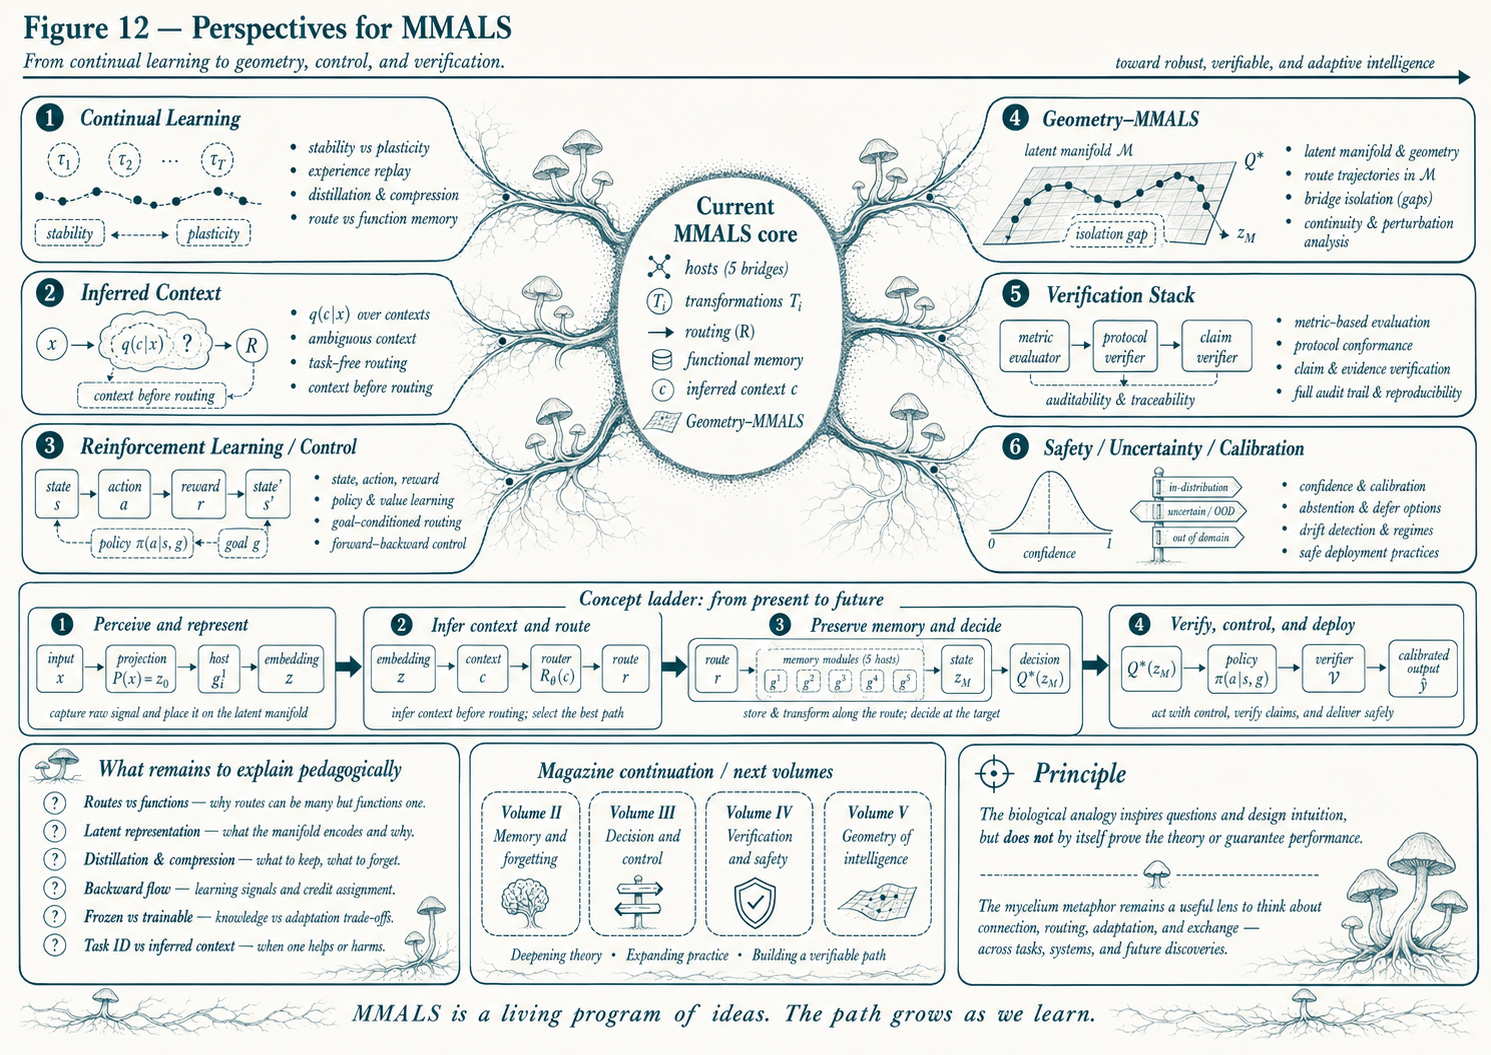
\includegraphics[width=0.985\linewidth,height=0.92\textheight,keepaspectratio]{assets/figure_perspectives_mmals.png}
\caption{Perspective map: continual learning, inferred context, reinforcement learning, geometry, verification and safe deployment.}
\end{figure}
\end{landscape}
\clearpage

\section{EcoSpec: keeping the research forest implementable}

EcoSpec is not another independent mechanism. It is a system contract designed to prevent architecture inflation. It unifies context, routes, memory, goals, health, budgets and audit into a minimal operational loop.

Its central design rule is:
\begin{keybox}
Use the simplest representation and control mechanism that preserves the information required for correct, stable, economical and auditable action.
\end{keybox}

The six normative axioms are:
\begin{enumerate}[leftmargin=1.6em]
\item systemic contribution;
\item functional memory;
\item deferred commitment;
\item sufficient simplicity;
\item goal-conditioned control;
\item earned complexity and falsifiable reduction.
\end{enumerate}

The three required operating modes are fast, ambiguous and critical. Advanced geometry, RL and density-state memory remain optional ablations that must reduce to the classical kernel and earn their cost.

\newpage
\section{What is established, plausible and still open?}

\begin{tabularx}{\textwidth}{p{3.2cm}X}
\toprule
\tablehead{Status} & \tablehead{Examples}\\
\midrule
Established inside the programme & Route identity is insufficient as a memory criterion; functional latent preservation is a meaningful diagnostic; context inference and evaluation timing materially affect results.\\
Supported but bounded & Some MMALS variants show strong retention in controlled protocols; Geometry-G1 shows a partial context-to-route functional bridge; RC2O-v2.3.1 shows old-context gains that fail full promotion gates.\\
Plausible research direction & Bottom-up host feedback, memory transport, goal-conditioned energy control, stable--plastic fusion and law-level drift diagnostics.\\
Not established & General MMALS superiority, positive backward transfer, stable causal host ecology, Riemannian-manifold claims, universal control, or quantum advantage.\\
\bottomrule
\end{tabularx}

\begin{researchbox}
A mature research programme is not weakened by blocked claims. It becomes stronger when negative results, failed gates and unexecuted designs remain visible.
\end{researchbox}

\section{Conclusion: learning to select, transform and preserve}

MMALS began with a forest metaphor: tree hosts connected through a fungal exchange system. The useful scientific content emerged only when the metaphor was converted into falsifiable objects: routes, transformations, contribution, cost, functional memory, context belief, drift, geometry, control and audit.

The most important internal lesson remains:
\[
\boxed{\text{The route is not the memory; the relevant memory is what the route computes.}}
\]
The next lesson is equally important:
\[
\boxed{\text{A memory is useful only if the system recognises when and why to activate it.}}
\]
And the system-level conclusion is:
\[
\boxed{\text{Complexity must be earned by evidence, uncertainty, risk, memory or goal.}}
\]

\section*{Documentary landmarks}
\addcontentsline{toc}{section}{Documentary landmarks}

\begin{itemize}[leftmargin=1.4em]
\item MMALS prototypes v0.1--v0.13.1: routing, fungal objectives, distillation, functional memory and co-evolution diagnostics.
\item MMALS Prototype v0.9: route--function disentanglement.
\item MMALS Prototype v0.11: comparative evidence harness.
\item A Mathematical Backbone for MMALS: distributional memory, optimal transport and information geometry.
\item Geometry-MMALS G1 v1.1.0: replicated context geometry to partial functional routing.
\item RC2O-v2.3.2 reviewer change report: per-sample stable--plastic context-fusion repair design.
\item MMALS EcoSpec 1.0: systemic TPUT specification and falsification ladder.
\end{itemize}

\end{document}
